% Chapter Template

\chapter{Results} % Main chapter title

\label{Chapter4} % Change X to a consecutive number; for referencing this chapter elsewhere, use \ref{ChapterX}

\lhead{Chapter 4. \emph{Results}} % Change X to a consecutive number; this is for the header on each page - perhaps a shortened title

In this section, we present the results obtained and the things we infer upon seeing the measurements. We measure the three key metrics, link utilization, RTT, packet loss along with the asymmetry and flow meta-data as described in the Methodology section and try to correlate them to prove congestion in the network.

\section{Trace collection}
The first strategy for collecting traces was to capture traffic at specific intervals of the day by running our capture tool and then analyzing the captured traffic. We wanted to check for congestion events in the network but this method didn't yield the results that we wanted. Since we were capturing traffic at random intervals, the probability of seeing a congestion event was very low. So we changed our strategy and captured traffic from 9 AM to 9 PM for the whole day on weekdays. The time at which we captured traffic was a recess week in the university, which implied that most of the students were not on campus. Figure \ref{fig:lu} shows the link utilization seen during the recess week during the busy hours,, which hardly touches $8Gbps$ sometimes. Hence, we again got low average link utilization throughout the day. We waited for the recess week to end and the examinations to begin. The traffic captured during the exam week showed high link utilization in general. The link utilization after the recess week is shown in figure \ref{fig:linkutilization}. Since the traffic was captured for 12 hours, the resultant pcap files were very large, accounting to over 500 GB of space on the server and time-consuming to process. So, we dissected the pcap files into smaller files of 10 min duration each using the editcap ~\cite{wireshark} tool from Wireshark.

\begin{figure}[t]
         \centering
         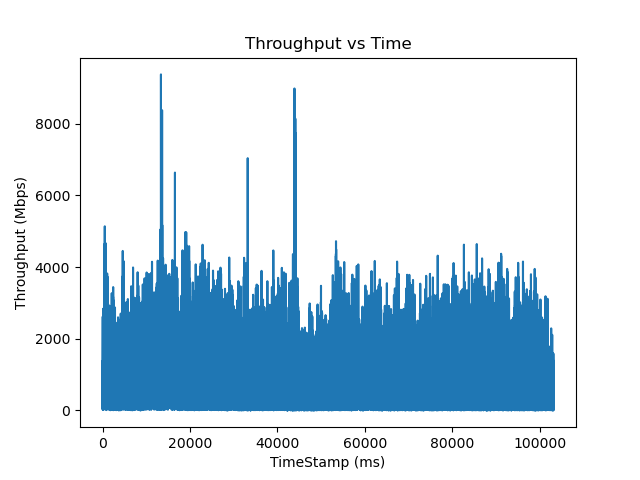
\includegraphics[width=0.6\textwidth]{Figures/link_util_11_29.png}
         \caption[Link utilization between 11:58 AM to 12:08 PM]{Link utilization between 11:58 AM to 12:08 PM}
         \label{fig:lu}
\end{figure}

\section{Link Utilization}
The link speed of the bottleneck link being tapped is $10Gbps$. If we see a saturation at $10Gbps$ for a prolonged period, we can state congestion as one of the possible reasons. We set the window size as 0.4 ms for calculating the throughput as already discussed. During peak hours, we saw saturation events for a prolonged period. Figures \ref{fig:linkutil1} and \ref{fig:linkutil2} show the link utilization during peak hours. The throughput almost constantly touches $10Gbps$ in both the traces. Figures \ref{fig:linkutil3} and \ref{fig:linkutil4} show the link utilization during non-peak hours where the throughput peaks at only some intervals and stays low for the rest of the time. The average link utilization throughout the day as seen from our measurements is around $6Gbps$, with the throughput only peaking during certain hours. Using Ookla's speed test we found out, that the network operators have rate-limited the download speed per machine to $100Mbps$. That means, there must be more than 100 concurrent users requesting data from the servers on the internet to exceed the link capacity of $10Gbps$. It is not expected that 100s of people simultaneously access data from the internet, hence the average link utilization staying low is not a surprising result. However, the link does get saturated around noon, the time when most of the lectures happen and people work in their labs.

\begin{figure}[t]
     \centering
     \begin{subfigure}[h]{0.49\textwidth}
         \centering
         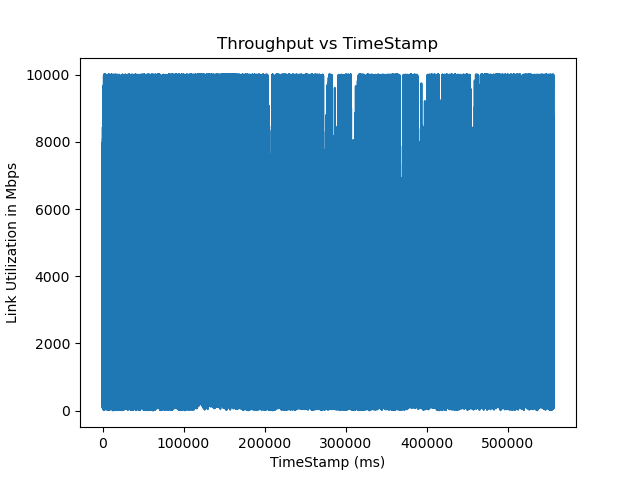
\includegraphics[width=\textwidth]{Figures/saturation_link_1.png}
         \caption[Link Utilization between 11:58 AM to 12:08 PM ]{Link Utilization between 11:58 AM to 12:08 PM}
         \label{fig:linkutil1}
     \end{subfigure}
     \begin{subfigure}[h]{0.49\textwidth}
         \centering
         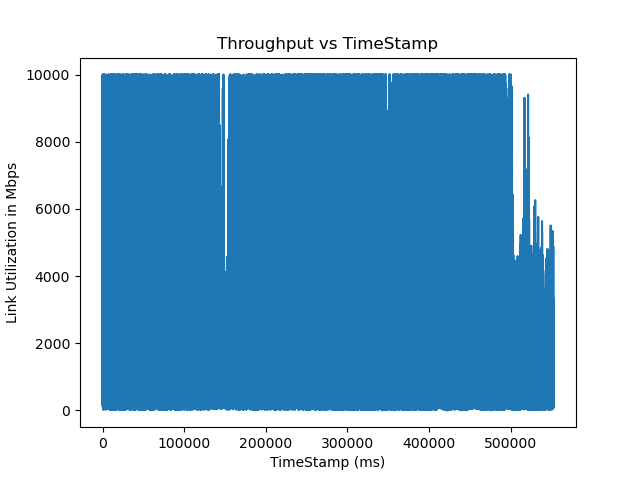
\includegraphics[width=\textwidth]{Figures/saturation_link_2.png}
         \caption[Link Utilization between 12:08 PM to 12:18 PM ]{Link Utilization between 12:08 PM to 12:18 PM }
         \label{fig:linkutil2}
     \end{subfigure}
     \begin{subfigure}[h]{0.49\textwidth}
         \centering
         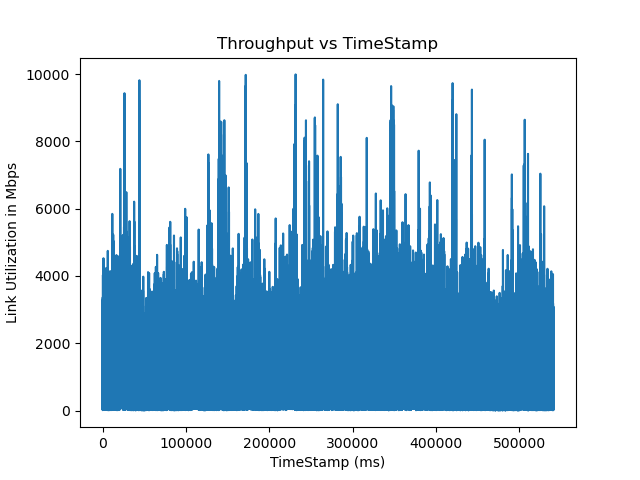
\includegraphics[width=\textwidth]{Figures/saturation_link_3.png}
         \caption[Link Utilization between 10:08 AM to 10:18 AM ]{Link Utilization between 10:08 AM to 10:18 AM }
         \label{fig:linkutil3}
     \end{subfigure}
     \begin{subfigure}[h]{0.49\textwidth}
         \centering
         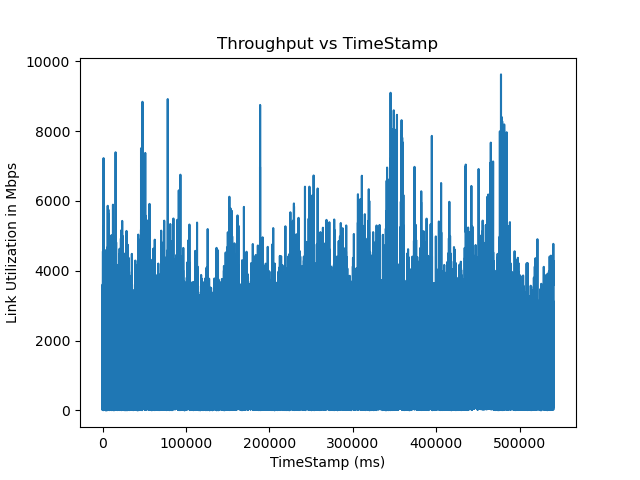
\includegraphics[width=\textwidth]{Figures/saturation_link_4.png}
         \caption[Link Utilization between 10:18 AM to 10:28 AM ]{Link Utilization between 10:18 AM to 10:28 AM }
         \label{fig:linkutil4}
     \end{subfigure}
     \bigskip
     \caption[Link Utilization during peak and non-peak hours]{Link Utilization during peak and non-peak hours}
     \label{fig:linkutilization}
     \bigskip
\end{figure}


%----------------------------------------------------------------------------------------

\section{RTT}
We measure the RTT for the internal leg of a flow using the algorithm discussed previously. The RTT is computed for all flows throughout their lifetime in the pcap trace. Figure \ref{fig:rttcomp} shows the internal leg of the RTTs for two traffic captures. For better understanding and visualizing the CDF, we've plotted the CDF of RTTs up to the 99th percentile. Figure \ref{fig:rtt1} has high RTT values with the 99th percentile recorded at 250ms because of saturation in the traffic capture, while figure \ref{fig:rtt2} has comparatively lower RTT values with the 99th percentile recorded at 102 ms. The RTT values indeed increase by a multiple of 2.5x in figure \ref{fig:rtt1} because of high link utilization, which results in packets getting queued in the buffer and the queueing delay factor being included in the RTT. We also measure the complete leg RTT of the flows using the TCP handshake as discussed previously. Figure \ref{fig:rttcomplete} shows the CDF of the complete-leg RTT values calculated using the TCP handshakes of the flows. These RTT values show a considerable shift in values since the studies done 20 years ago~\cite{tcprtt-imc03}. ~\cite{tcprtt-imc03} states that around 50\% of the RTT samples have RTT lesser than 100ms, whereas our CDF shows that 50\% of the flows have their RTTs lesser than 2ms. The previous studies also reported 90\% of the flows to be having RTT values lesser than 1s, whereas our measurements state that 90\% of the flows have their RTTs lesser than 200ms. These results show that the RTT values have decreased by a huge factor since the last studies done because of several reasons like CDNs and faster links in the backbone of the internet. Our measurements thus contribute to replenishing the old RTT measurements.

\begin{figure}[t]
     \centering
     \begin{subfigure}[h]{0.49\textwidth}
         \centering
         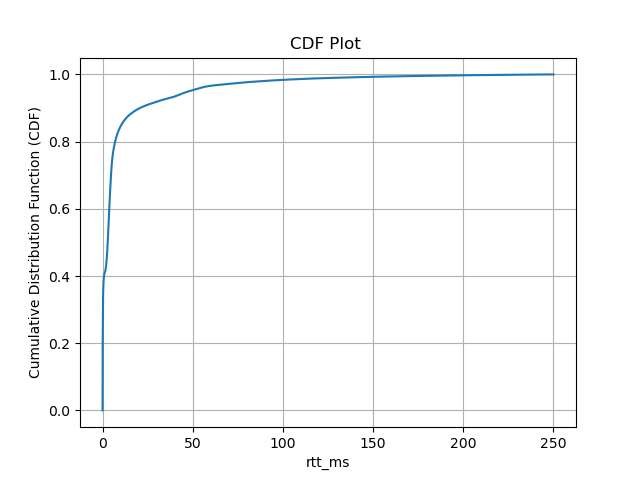
\includegraphics[width=\textwidth]{Figures/rtt_cdf 1.png}
         \caption[CDF of RTT for a saturated traffic capture]{CDF of RTT for a saturated traffic capture}
         \label{fig:rtt1}
     \end{subfigure}
     \begin{subfigure}[h]{0.49\textwidth}
         \centering
         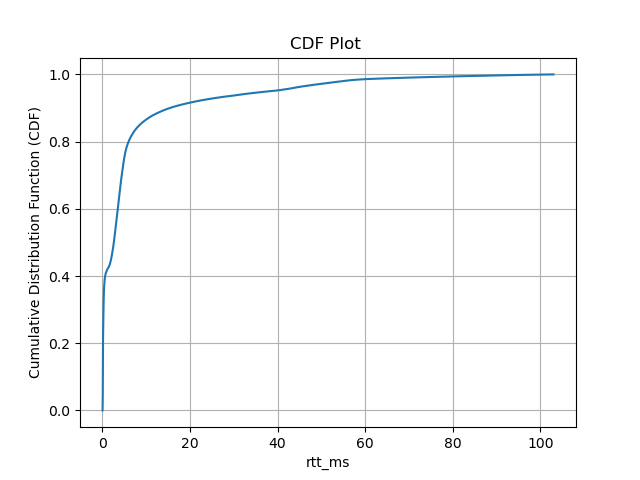
\includegraphics[width=\textwidth]{Figures/rtt_cdf1.png}
         \caption[CDF of RTT for a normal traffic capture]{CDF of RTT for a normal traffic capture}
         \label{fig:rtt2}
     \end{subfigure}
     \caption[Comparison of CDF of RTTs for different traffic captures]{Comparison of CDF of RTTs for different traffic captures}
     \label{fig:rttcomp}
     \bigskip
\end{figure}

\begin{figure}[t]
    \centering
        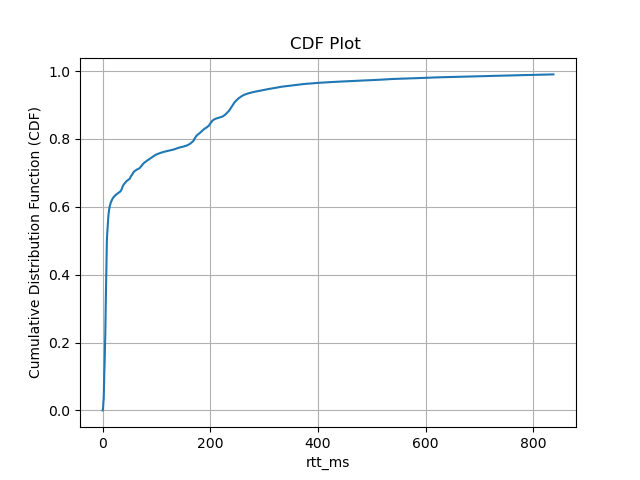
\includegraphics[width=0.6\textwidth]{Figures/complete_rtt.png}
    \caption[CDF of complete leg RTT for a trace]{CDF of complete leg RTT for a trace}
    \label{fig:rttcomplete}
    \bigskip
\end{figure}

%----------------------------------------------------------------------------------------
\section{Packet Loss}

We plot packet losses for a trace by marking the point at which a packet loss happened with a vertical line in Figure~\ref{fig:pktloss}. We mark internet side losses with a red vertical line and the campus(SoC) side losses with a blue vertical line.  One of the possible reasons for packet losses on the campus side being higher in this snapshot might be due to higher losses in the wireless network as compared to the wired network. The average loss rate on the SoC side is seen to be around 0.3\% of the total packets. The packet loss on the internet side for the traces showing high link utilization is lesser than 1\%, somewhere around 0.7\%. The packet losses for the traces showing lower link utilization are higher than 1\% in general. These results make sense because higher packet losses will force flows to decrease their congestion window sizes, which would decrease per-flow throughput leading to lower link utilization. The number of re-ordering events in the network is very large, with around 3-4\% of the total packets getting re-ordered, which compels us to put a check on the time difference between the appearance of the hole in the sequence number chain, and the actual appearance of the packet. The number of packets lost on the internet side may appear to be higher than usual because the time difference currently being considered is kept equal to the RTT of the flow, but some re-ordered packets might arrive later than an RTT because of taking a longer path in the network, but are being counted as packet losses on the internet side. 

\begin{figure}[t]
    \centering
        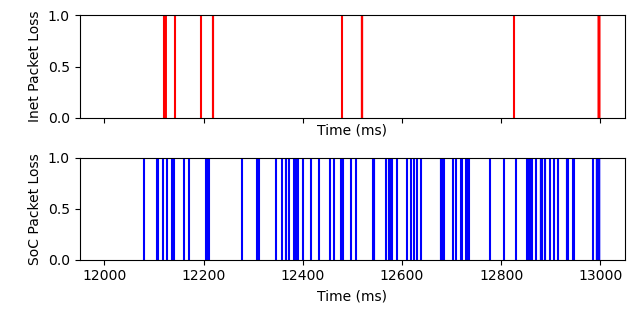
\includegraphics[width=0.75\textwidth]{Figures/packetloss.png}
    \caption[Packet Losses for a trace]{Packet Losses for a trace}
    \label{fig:pktloss}
    \bigskip
\end{figure}

\section{Asymmetry}

We aim to find the number of asymmetric flows in our captures to make sure that our calculations involving both the downlink and uplink pcap files are correct. Let's say a flow $f$ is asymmetric. While calculating the RTT for a capture, we will miss the ACK for some packets of the flow $f$  and it may result in the average RTT being reported wrongly. We find after running our scripts that the number of asymmetric flows is always lesser than 10\% and on average around 7\%. 
Since the number of asymmetric flows is not large, we are able to measure the RTTs of almost all the packets.
%----------------------------------------------------------------------------------------

\section{Other Flow Metrics}

\begin{figure}[t]
    \centering
        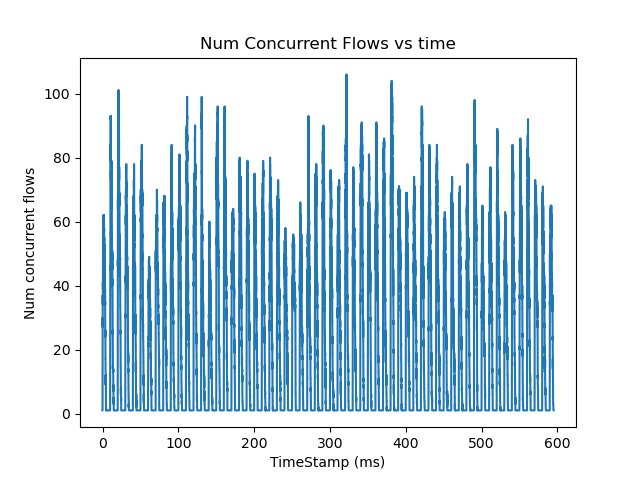
\includegraphics[width=0.75\textwidth]{Figures/concurrent_flows.png}
    \caption[Number of Concurrent Flows]{Number of Concurrent Flows}
    \label{fig:concurr}
    \bigskip
\end{figure}

Figure \ref{fig:concurr} shows the plot of the number of concurrent flows vs time for one of the traffic captures. The number of concurrent flows is an important meta-data used in designing new algorithms. The graph shows that the maximum number of concurrent flows at any point of time is 106. If we are designing a new algorithm for AQM, the metric of the number of concurrent flows will be handy for deciding the number of queues required to accommodate all the flows.

\begin{figure}[t]
    \centering
        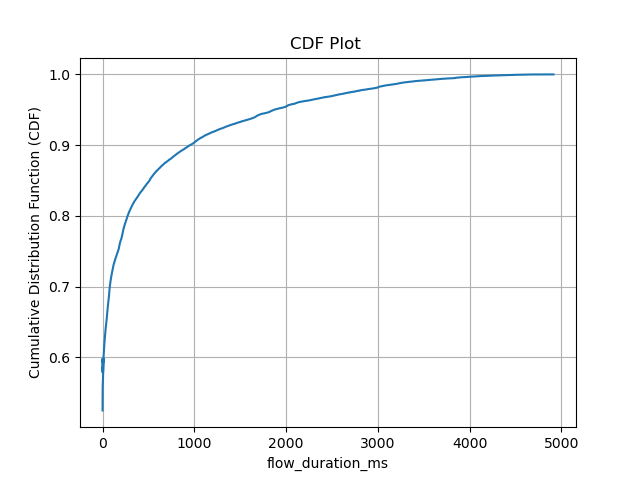
\includegraphics[width=0.75\textwidth]{Figures/flow_duration_cdf.png}
    \caption[Flow duration in ms]{Flow Duration in ms}
    \label{fig:dur}
    \bigskip
\end{figure}

Figure \ref{fig:dur} shows the cdf of the flow duration for the pcap trace. We see from the graph that 60\% of the flows have a duration very close to 0 ms. This tells us that most of the flows are short-lived. Other than that, 90\% of the flows have a duration of less than 1s, and only 10\% of the flows have their  \( duration > 1s \)  with the maximum flow duration being $5s$. Flow duration is another important meta-data that gives us information about the lifetime of a flow, and gives us the proportion of the number of short and long flows in the network which helps us in understanding the network composition better.

\begin{figure}[t]
     \centering
     \begin{subfigure}[h]{0.49\textwidth}
         \centering
         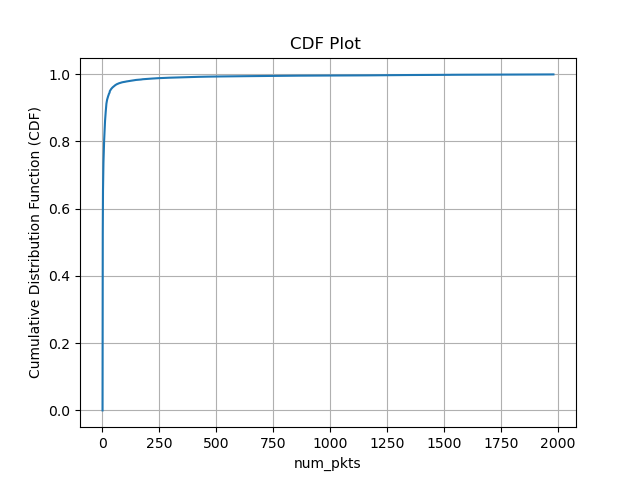
\includegraphics[width=\textwidth]{Figures/num_pkts_cdf.png}
         \caption[CDF of number of packets of flows]{CDF of number of packets of flows}
         \label{fig:pkts1}
     \end{subfigure}
     \begin{subfigure}[h]{0.49\textwidth}
         \centering
         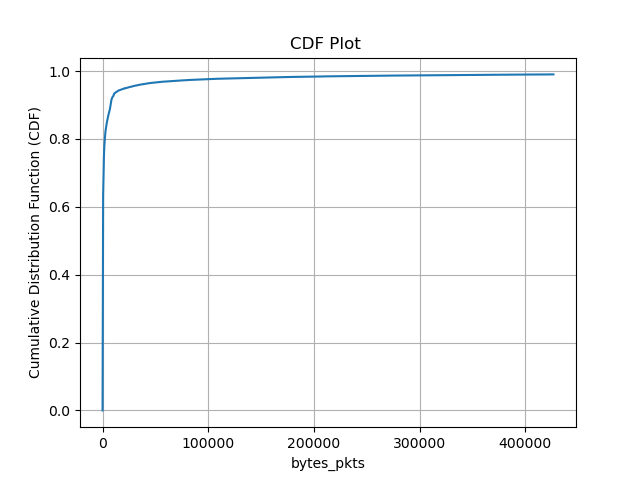
\includegraphics[width=\textwidth]{Figures/byte_pkts_cdf.png}
         \caption[CDF of number of bytes of flows]{CDF of number of bytes of flows}
         \label{fig:pkts2}
     \end{subfigure}
     \caption[Flow sizes]{Flow sizes}
     \label{fig:pktcdf}
     \bigskip
\end{figure}

Figure \ref{fig:pktcdf} shows the cdf of the number of packets of flows \ref{fig:pkts1} and the number of bytes of flows \ref{fig:pkts2}. As seen from figure \ref{fig:dur} of the flow durations, most of the flows are short lived. Hence, it is imperative that sizes of most of the flows will be small. The CDFs show that around 90\% of the flows have number of packets smaller than 250 and he number of bytes smaller than 7500 bytes. Hence, from these graphs we get to know that most of the flows in the network are short-lived with small flow sizes.



%----------------------------------------------------------------------------------------

\section{Correlation between Link Utilization,Packet Loss and RTT}

We consider a pcap trace which has both regions of high link utilization and low link utilization to show congested regions. Figure \ref{fig:linkutil_satur} shows the pcap trace being considered for the correlation. The pcap trace experiences a high jump in link utilization around the 400s mark. If we see a correspondence between the RTT, link utilization and packet losses around this point, we'll be able to pinpoint a congestion event.

We want to consider a flow, which exists in both regions of low link utilization and high link utilization and see how different metrics of the flow change when it goes through this transition. Figure \ref{fig:corr} shows the correlation between the RTT values of one of such flows and the link utilization. \ref{fig:corr} shows that the RTT values of the flow experience a spike as soon as the link utilization starts touching $10Gbps$ and the RTT increases in general through the high link utilization region.Since we are monitoring the internal leg RTT, the graph suggests that there is congestion inside the campus network as the RTT values of the internal leg are increasing.

Figure \ref{fig:correlation} further shows the packet losses along with the RTT and link utilization. As the link utilization increases, the RTT values of a flow being monitored increase continuously and a cluster of packet losses on the internet side is also seen. This graph, on the contrary, suggests that congestion is happening on the internet side due to an increase in packet losses on the internet side. The packet losses happen due to buffer overflow in a congested link before the campus. 

These results show the occurrence of congestion, but locating the point of congestion requires further study.

\begin{figure}[t]
    \centering
        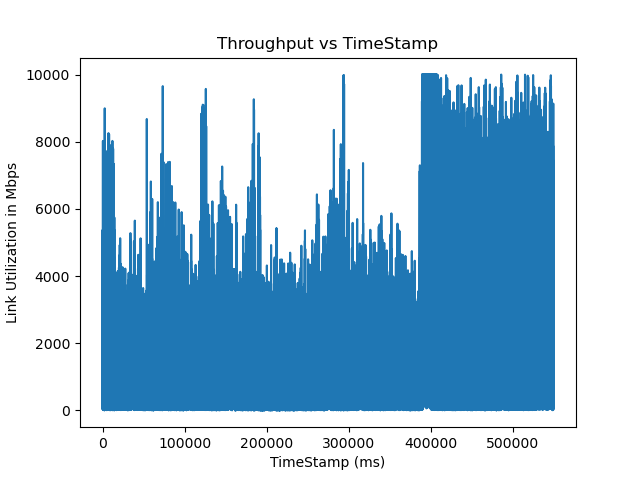
\includegraphics[width=0.75\textwidth]{Figures/link_util_satur.png}
    \caption[Link Utilization of the trace being considered]{Link Utilization of the trace being considered}
    \label{fig:linkutil_satur}
    \bigskip
\end{figure}

\begin{figure}[t]
    \centering
        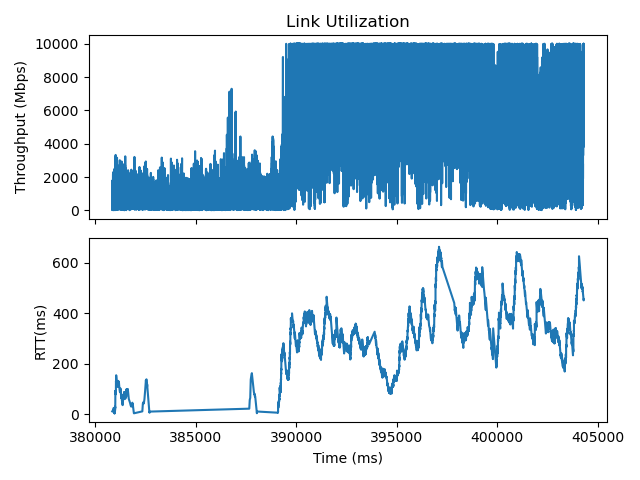
\includegraphics[width=0.75\textwidth]{Figures/RTT_saturation.png}
    \caption[Correlation between RTT of a flow and link utilization]{Correlation between RTT of a flow and link utilization}
    \label{fig:corr}
    \bigskip
\end{figure}

\begin{figure}[t]
    \centering
        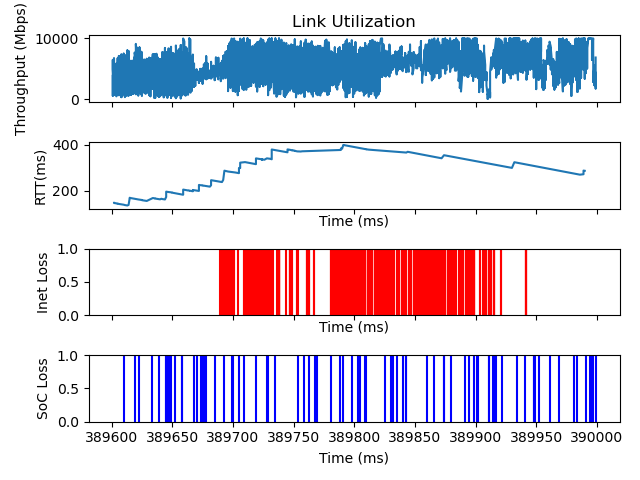
\includegraphics[width=0.75\textwidth]{Figures/correlation.png}
    \caption[Correlation between RTT,link utilization and packet loss]{Correlation between RTT,link utilization and packet loss}
    \label{fig:correlation}
    \bigskip
\end{figure}

%----------------------------------------------------------------------------------------